
\documentclass[border=10pt, 12pt]{standalone}
\usepackage[svgnames]{xcolor}
\usepackage{amsmath}
\usepackage{pgfplots}
\pgfplotsset{compat=newest}
\usepackage[sfdefault]{FiraSans}
\usepackage{FiraMono}
\renewcommand*\familydefault{\sfdefault}
\begin{document}
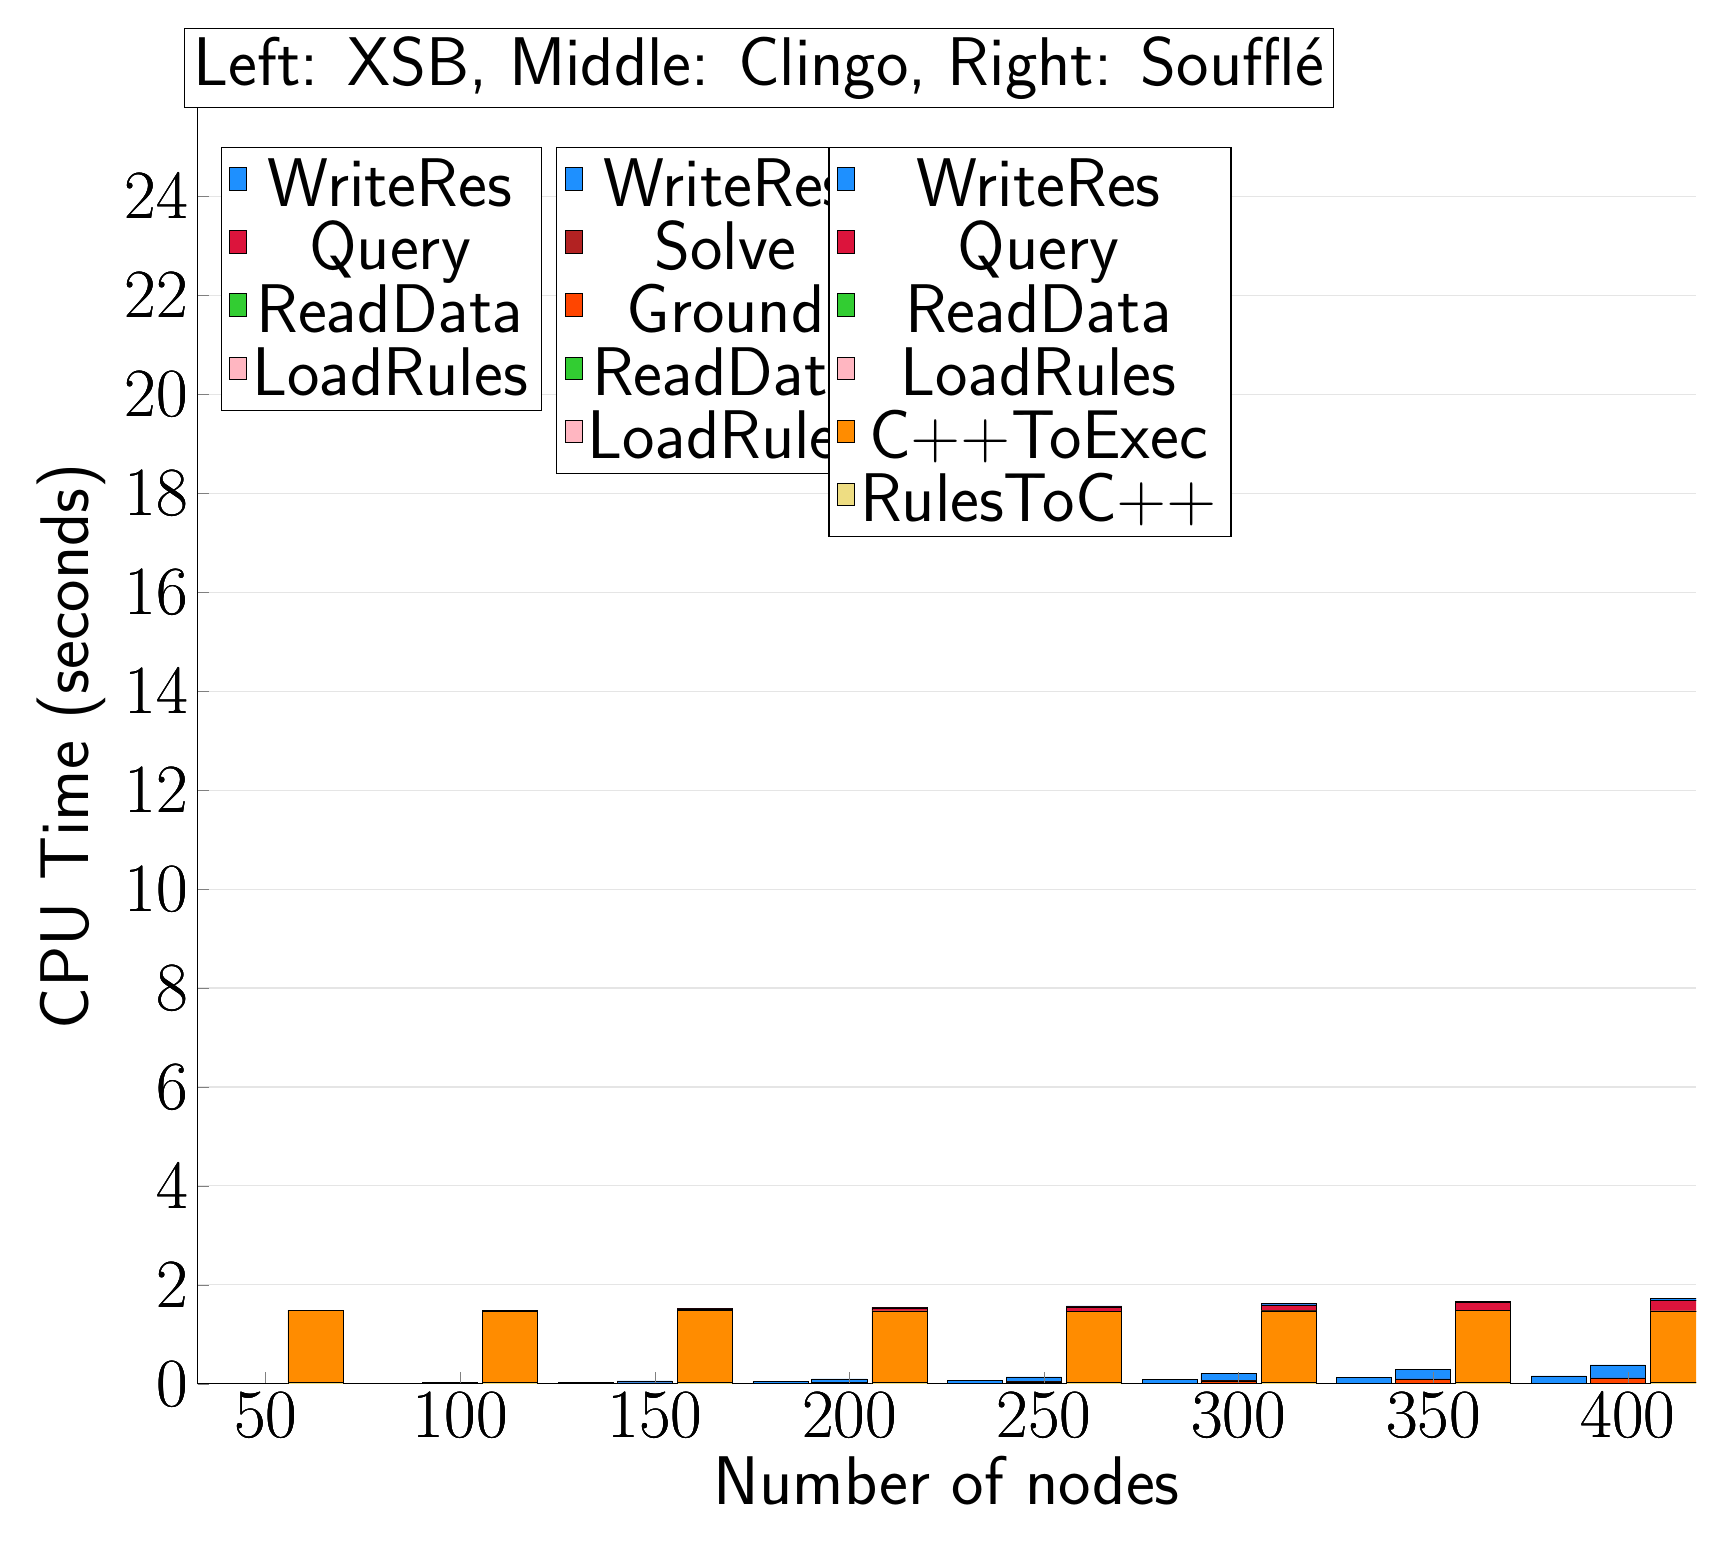
\begin{tikzpicture}
	\begin{axis}[bar shift=-25pt,
			ybar stacked,
			width=1.7\textwidth,
			bar width=0.7cm,
			ymajorgrids, tick align=inside,
			major grid style={draw=gray!20},
			xtick=data,
			ymin=0, ymax=25.779619999999998,
			axis x line*=bottom,
			axis y line*=left,
			enlarge x limits=0.05,
			legend style={
					at={(0.23, 0.97)},
					anchor=north east,
					legend columns=1,
					font=\Huge,
				},
			ylabel={CPU Time (seconds)},
			xlabel={Number of nodes},
			label style={font=\Huge},
			tick label style={font=\Huge},
		]
		\addlegendimage{fill=DodgerBlue, draw=black, line width=0.2pt}
		\addlegendentry{WriteRes}
		\addlegendimage{fill=Crimson, draw=black, line width=0.2pt}
		\addlegendentry{Query}
		\addlegendimage{fill=LimeGreen, draw=black, line width=0.2pt}
		\addlegendentry{ReadData}
		\addlegendimage{fill=LightPink, draw=black, line width=0.2pt}
		\addlegendentry{LoadRules}
		\addplot +[fill=LightPink, draw=black, line width=0.2pt] coordinates {
				(50, 0.0006333)
				(100, 0.0005995)
				(150, 0.0006054)
				(200, 0.0006274999999999999)
				(250, 0.0006001000000000001)
				(300, 0.0006181999999999998)
				(350, 0.0006144999999999998)
				(400, 0.0006131000000000004)
			};
		\addplot +[fill=LimeGreen, draw=black, line width=0.2pt] coordinates {
				(50, 0.0001802999999999996)
				(100, 0.0002196999999999999)
				(150, 0.00026230000000000014)
				(200, 0.0003135999999999998)
				(250, 0.00035130000000000024)
				(300, 0.00039990000000000007)
				(350, 0.00044700000000000046)
				(400, 0.0004748999999999993)
			};
		\addplot +[fill=Crimson, draw=black, line width=0.2pt] coordinates {
				(50, 0.0002576999999999999)
				(100, 0.0009696999999999998)
				(150, 0.0021565)
				(200, 0.0038309999999999998)
				(250, 0.005784600000000001)
				(300, 0.0087443)
				(350, 0.0119166)
				(400, 0.015354399999999999)
			};
		\addplot +[fill=DodgerBlue, draw=black, line width=0.2pt] coordinates {
				(50, 0.0023225000000000003)
				(100, 0.009300600000000001)
				(150, 0.0209035)
				(200, 0.036817)
				(250, 0.0573877)
				(300, 0.08264429999999999)
				(350, 0.1128278)
				(400, 0.1456286)
			};
	\end{axis}

	\begin{axis}[bar shift=-3.7pt,
			ybar stacked,
			width=1.7\textwidth,
			bar width=0.7cm,
			ymajorgrids, tick align=inside,
			major grid style={draw=none},
			xtick=data,
			ymin=0, ymax=25.779619999999998,
			axis x line*=none,
			axis y line*=none,
			enlarge x limits=0.05,
			legend style={
					at={(0.454, 0.97)},
					anchor=north east,
					legend columns=1,
					font=\Huge,
				},
			label style={font=\Huge},
			tick label style={font=\Huge},
		]
		\addlegendimage{fill=DodgerBlue, draw=black, line width=0.2pt}
		\addlegendentry{WriteRes}
		\addlegendimage{fill=FireBrick, draw=black, line width=0.2pt}
		\addlegendentry{Solve}
		\addlegendimage{fill=OrangeRed, draw=black, line width=0.2pt}
		\addlegendentry{Ground}
		\addlegendimage{fill=LimeGreen, draw=black, line width=0.2pt}
		\addlegendentry{ReadData}
		\addlegendimage{fill=LightPink, draw=black, line width=0.2pt}
		\addlegendentry{LoadRules}
		\addplot +[fill=LightPink, draw=black, line width=0.2pt] coordinates {
				(50, 0.0)
				(100, 0.0)
				(150, 0.0)
				(200, 0.0)
				(250, 0.0)
				(300, 0.0)
				(350, 0.0)
				(400, 0.0)
			};
		\addplot +[fill=LimeGreen, draw=black, line width=0.2pt] coordinates {
				(50, 0.0)
				(100, 0.0)
				(150, 0.0)
				(200, 0.0)
				(250, 0.0)
				(300, 0.0)
				(350, 0.0)
				(400, 0.0)
			};
		\addplot +[fill=OrangeRed, draw=black, line width=0.2pt] coordinates {
				(50, 0.0)
				(100, 0.009999999999999997)
				(150, 0.019999999999999997)
				(200, 0.030000000000000006)
				(250, 0.03999999999999999)
				(300, 0.06000000000000001)
				(350, 0.08799999999999998)
				(400, 0.11000000000000001)
			};
		\addplot +[fill=FireBrick, draw=black, line width=0.2pt] coordinates {
				(50, 0.0)
				(100, 0.0)
				(150, 0.0)
				(200, 0.0)
				(250, 0.010000000000000009)
				(300, 0.009999999999999995)
				(350, 0.011999999999999993)
				(400, 0.012000000000000005)
			};
		\addplot +[fill=DodgerBlue, draw=black, line width=0.2pt] coordinates {
				(50, 0.009999999999999997)
				(100, 0.020000000000000007)
				(150, 0.038)
				(200, 0.06999999999999998)
				(250, 0.08999999999999998)
				(300, 0.139)
				(350, 0.18999999999999997)
				(400, 0.25999999999999995)
			};
	\end{axis}

	\begin{axis}[bar shift=18pt,
			ybar stacked,
			width=1.7\textwidth,
			bar width=0.7cm,
			ymajorgrids, tick align=inside,
			major grid style={draw=none},
			xtick=data,
			ymin=0, ymax=25.779619999999998,
			axis x line*=none,
			axis y line*=none,
			enlarge x limits=0.05,
			legend style={
					at={(0.69, 0.97)},
					anchor=north east,
					legend columns=1,
					font=\Huge,
				},
			label style={font=\Huge},
			tick label style={font=\Huge},
		]
		\addlegendimage{fill=DodgerBlue, draw=black, line width=0.2pt}
		\addlegendentry{WriteRes}
		\addlegendimage{fill=Crimson, draw=black, line width=0.2pt}
		\addlegendentry{Query}
		\addlegendimage{fill=LimeGreen, draw=black, line width=0.2pt}
		\addlegendentry{ReadData}
		\addlegendimage{fill=LightPink, draw=black, line width=0.2pt}
		\addlegendentry{LoadRules}
		\addlegendimage{fill=DarkOrange, draw=black, line width=0.2pt}
		\addlegendentry{C++ToExec}
		\addlegendimage{fill=LightGoldenrod, draw=black, line width=0.2pt}
		\addlegendentry{RulesToC++}
		\addplot +[fill=LightGoldenrod, draw=black, line width=0.2pt] coordinates {
				(50, 0.031000000000000007)
				(100, 0.030000000000000006)
				(150, 0.030000000000000006)
				(200, 0.030000000000000006)
				(250, 0.030000000000000006)
				(300, 0.030000000000000006)
				(350, 0.030000000000000006)
				(400, 0.030000000000000006)
			};
		\addplot +[fill=DarkOrange, draw=black, line width=0.2pt] coordinates {
				(50, 1.446)
				(100, 1.4389999999999998)
				(150, 1.451)
				(200, 1.4449999999999998)
				(250, 1.4399999999999997)
				(300, 1.4460000000000002)
				(350, 1.4489999999999998)
				(400, 1.4439999999999997)
			};
		\addplot +[fill=LightPink, draw=black, line width=0.2pt] coordinates {
				(50, 2.5300000000000002e-05)
				(100, 0.0)
				(150, 1.11e-05)
				(200, 1.01e-05)
				(250, 1.09e-05)
				(300, 1.09e-05)
				(350, 1.1e-05)
				(400, 1.11e-05)
			};
		\addplot +[fill=LimeGreen, draw=black, line width=0.2pt] coordinates {
				(50, 0.0004142)
				(100, 0.0005162)
				(150, 0.0006143)
				(200, 0.0007325)
				(250, 0.0008121000000000002)
				(300, 0.0008624000000000001)
				(350, 0.0010308)
				(400, 0.0011068999999999999)
			};
		\addplot +[fill=Crimson, draw=black, line width=0.2pt] coordinates {
				(50, 0.0043143)
				(100, 0.0159942)
				(150, 0.03501230000000001)
				(200, 0.0576405)
				(250, 0.08530890000000001)
				(300, 0.11729890000000001)
				(350, 0.1592501)
				(400, 0.20581960000000002)
			};
		\addplot +[fill=DodgerBlue, draw=black, line width=0.2pt] coordinates {
				(50, 0.0013817)
				(100, 0.0039406)
				(150, 0.0074017)
				(200, 0.011368800000000002)
				(250, 0.017483199999999997)
				(300, 0.025026399999999997)
				(350, 0.0343169)
				(400, 0.045253400000000006)
			};
	\end{axis}


	\node[anchor=south, draw, fill=white] at (rel axis cs:0.42,1) {\Huge Left: XSB, Middle: Clingo, Right: Soufflé};
\end{tikzpicture}
\end{document}
